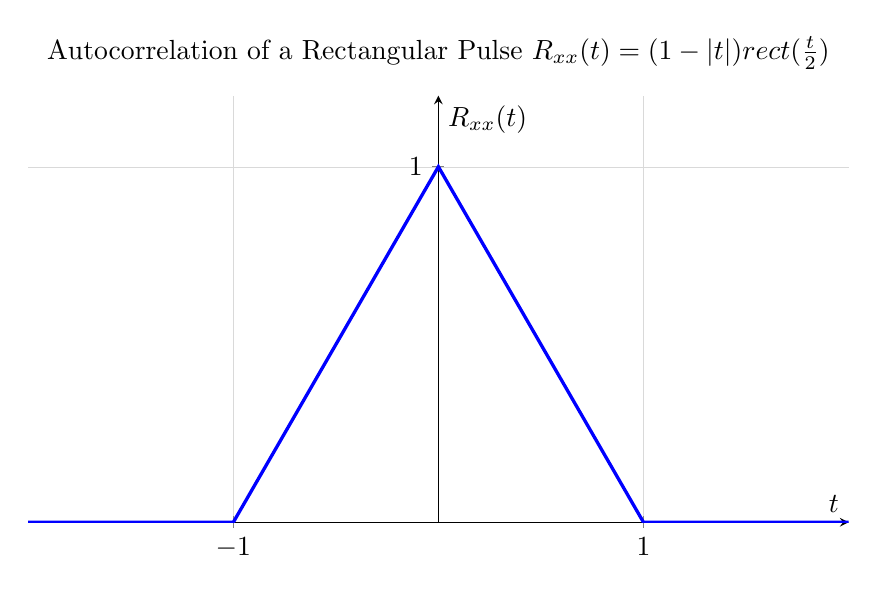
\begin{tikzpicture}
	\begin{axis}[
		width=12cm,
		height=7cm,
		title={Autocorrelation of a Rectangular Pulse $R_{xx}(t) = (1-|t|) \text{rect}(\frac{t}{2})$},
		xlabel={$t$},
		ylabel={$R_{xx}(t)$},
		axis lines=middle,
		xmin=-2, xmax=2,
		ymin=0, ymax=1.2,
		xtick={-1, 1},
		ytick={1},
		grid=major,
		grid style={line width=.1pt, draw=gray!30},
		]
		\draw[blue, very thick]
		(axis cs:-2,0) -- (axis cs:-1,0) -- (axis cs:0,1) 
		-- (axis cs:1,0) -- (axis cs:2,0);
	\end{axis}
\end{tikzpicture}